\chapter{Calculating Temperature Changes using the fMRI BOLD Response}
    
  \section{\label{sec:tempmodelintro} Introduction}
  Current efforts to model temperature changes be can categorized into two classes.  The first class approaches the problem by considering a single voxel deep within the brain (single-voxel approach) while the second approach considers the brain and head as an entire system (multi-voxel approach).  Each of these methods has their own pros and cons which will be discussed below.
  %%  SINGLE VOXEL APROACH %%
    \subsection{\label{sec:singlevox} Single-Voxel Approach}
    A single-voxel model of temperature was first proposed by SOMEONE, but has been refined over the past HOWLONG years CITEABUNCH to include more terms.  Although different approaches consider different contributions to the temperature change, they all narrow the problem down to a single voxel which is usually 2mm x 2mm x 2mm.  By simplifying the model, the heat equation can be simplified and the calculation is much easier to undertake.  However, since the brain is not homogenous, the values used for parameters such as heat production and thermal conductivity are taken from an average of the tissues.  As a result, this reduces the possible accuracy of such a model when applied to a subject.
    
    The most recently published iteration of a single-voxel model was published by~\citet{sotero2011}.  The basis of this model is a modification of the Penne's Bioheat Equation~\citep{pennes, sotero2011}.
    %%%%%%%  Bio-heat Equation %%%%%%%%%%%%
    \begin{align}
      \label{eq:bioheat}
      C_t \frac{dT(t)}{dt} &= (\Delta H^{\circ}-\Delta H_{b}) CMRO_{2}\mid_{0} m(t) - \rho_{b} C_{b} CBF\mid_{0} f(t) (T(t) - T_{a}) \nonumber \\
      &\qquad {} - \frac{C_{t}}{\tau} (T(t)-T_{0})
    \end{align}
    where $C_t$ is the specific heat of the tissue, $\Delta H^{\circ}$ is the enthalpy released in the oxidation of glucose, $\Delta H_b$ is the enthalpy used to release oxygen from hemoglobin, $COMRO_2 \mid_0$ is the metabolic rate at rest, $\rho_b$ is the blood density, $C_b$ is the specific heat of blood, $CBF\mid_0$ is the cerebral blood flow at rest, $T_a$ is the arterial blood temperature, $C_T$ is the specific heat for the tissue, and $\tau$ is a time constant for conductive heat loss.  The values used are provided in~\cref{tbl:soteroparams}.
    
    One advantage of using~\cref{eq:bioheat} is that the resting state temperature can be analytically determined by substituting $\frac{dT(t)}{dt} = 0$~\citep{sotero2011}.
    %%%%%%%  Resting state temperature %%%%%
    \begin{equation}
      \label{eq:restingtemperature}
      T_{0} = T_{a} + \frac{(\Delta H \mid^{\circ} - \Delta H_{b}) CMRO_{2}\mid_{0}}{\rho_{B} C_{B} CBF\mid_{0}}
    \end{equation}
    If the values provided in~\cref{tbl:soteroparams} are substitued into~\cref{eq:restingtemperature}, a resting temperature of 37.3057\degree C is found.  Since the resting temperature is always greater than the arterial blood temperature, it limits the ability of the model to account for all experimental results. 
    
    While~\cref{eq:bioheat} is appears complicated, conceptually the equation can be easily understood.
    %%%%%%%  Explanation %%%%%%%%%%%%%%%%%%%
    \begin{align}    
      \label{eq:soteroexplaiend}
      change\ in\ temperature\ &=\ heat\ generated\ by\ metabolism\ -\ heat\ lost\ to\ convection\ \nonumber \\
      &\qquad {} -\ heat\ lost\ to\ conduction
    \end{align}
    The system is a balance between heat generation (metabolism) and heat transfer (conduction and convection).  The direction of heat transfer by convection is determined by the difference between the voxel temperature and the arterial blood temperature ($T(t) - T_a$).  Similarly, the direction of heat transfer by conduction is determined by the difference between the voxel temperature and the temperature of the surrounding tissue ($T(t) - T_0$).  Since $T_a$ is less than $T(0)$, an increase in blood flow ($f(t)$) will remove heat from the voxel thereby decreasing the temperature.  Conversely, an increase in metabolism ($m(t)$) without a corresponding change in blood flow, will result in tissue warming.  
    
    %%  MULTI VOXEL APPROACH  %%
    \subsection{\label{sec:multivox} Multi-Voxel Approach}
    The multi-voxel approach to calculating brain tissue temperature alleviates many of the issues that a single-voxel approach has.  The most prominent advantage a multi-voxel approach has is the a result of it accounting for a voxels location relative to the surface of the head and other voxels.  By accounting for a voxel's location, the same BOLD response in two different locations can have vastly different effects on the local tissue temperature (more on this in~\cref{sec:theoreticalresults}).
    At the heart of our method is a three-dimensional implementation of the Pennes bioheat equation (\cref{eq:3dbioheat})\citep{collins}.
    \begin{equation} \label{eq:3dbioheat} 
    	\rho c \frac{dT}{dt} = k \nabla^{2}T-\rho_{blood}f(t)wc_{blood}(T-T_{blood})+m(t)Q_{m} 
    \end{equation}
  where $\rho$ is the tissue density, $c$ is the specific heat of the voxel, $k$ is the thermal conductivity, $\rho_{blood}$ is the blood density, $w$ is perfusion by blood, $c_{blood}$ is the specific heat of blood, $T_{blood}$ is the arterial blood temperature, and $Q_{m}$ is the baseline metabolic heat production. $f(t)$ and $m(t)$ are the time-dependent changes in blood flow and metabolism. These two factors determine the short-term change in temperature and are calculated from the fMRI BOLD response (see~\cref{sec:approach} for more on this).

% THE APPROACH
\section{Our Approach}
  \label{sec:approach}
  The fundamental difference between our temperature modeling approach and the single-voxel models discussed in~\cref{sec:tempmodelintro} is that we consider the entire head. The Pennes bioheat equation (\cref{eq:bioheat}) \citep{pennes,sotero2011} includes three terms. The first and second terms describe heat generation by metabolism and heat exchange by convection to blood flow.  On shorter time scales, these two terms dominate and are sufficient for determining the temperature change; however, the third term becomes important on longer time scales.
  
  The third term describes the heat exchanged by conduction to surrounding tissues.  This is a comparatively slow process, but on larger time scales determines the resting state temperature.  When calculating the temperature change, it is important to first have an accurate resting state temperature.  By considering the entire head, out model is able to accurately determine a resting state temperature for each voxel, enabling far more accurate temperature calculations than what is capable with single-voxel approaches.  \Cref{fig:procedureflowchart} gives a schematic of the temperature calculation procedure.
  
  [WRITE SOMETHING HERE]
    
  \begin{figure}[tb]
    \caption[Procedure used to calculate temperature change]{\label{fig:procedureflowchart} The procedure used to calculate temperature from BOLD data.  Orange blocks ($\color{goldfish}\bullet$) represent data, the sandy-colored block ($\color{beachstorm}\bullet$) is a step done using SPM8 and the teal blocks ($\color{aoi}\bullet$) are steps done using a function provided within temptools (\cref{appendix:code}).}
    \vspace{10pt}
    \centering
    \tikzstyle{data} = [draw=none, fill=goldfish]
\tikzstyle{temptools} = [draw=none, fill=aoi]
\tikzstyle{spm} = [draw=none, fill=beachstorm]
\tikzstyle{params} = [draw=none, fill=pondwater]
\tikzstyle{line} = [draw, very thick, color=black!50, -stealth']

\begin{tikzpicture}[node distance=0.7cm, rectangle, text width=4.5cm, text badly centered, rounded corners, minimum height=1cm, anchor=north]     
  % Left column
    \node[data](fmridata){fMRI BOLD Data};
    \node[temptools, below=of fmridata](calcrest){Calculate resting state (avg\_NII\_rest)};
    \node[temptools, below=of calcrest](normalize){Normalize the data to resting state (avg\_NII\_normalize)};
    \node[temptools, below=of normalize](boldtomf){Calculate the change in metabolism and blood flow (BOLDtoMF)\\Details given in \cref{sec:calcmf}};
    % middle column
    \node[data, right=of fmridata](t1contrast){T1 contrast image};
    \node[spm, below=of t1contrast](segment){Segment image (SPM8)};
    \node[temptools, right=of boldtomf](buildhead){Build head matrix (ImportSegmentedT1)\\Details given in \cref{sec:prephead}};
    % right column
    \node[temptools, right=of buildhead](calcequil){Calculate equilibrium temperature (tempCalcEquilibrium)\\Details given in \cref{sec:calcequilT}};
    \node[params, above=of calcequil, xshift=-2cm](tissueparams){Tissue-specific parameters (given in \cref{tbl:tissues})};
    % bottom
    \node[temptools, below=of buildhead, text width=8cm](calctemp){Find temperature change during activity (tempCalcDynMF)\\Details given in \cref{sec:calcT}};
  
  \path[line](fmridata) -- (calcrest);
  \path[line](calcrest) -- (normalize);
  \path[line](normalize) -- (boldtomf);
  \path[line](t1contrast) -- (segment);
  \path[line](segment) -- (buildhead);
  \path[line](buildhead) -- (calcequil);
  \path[line](boldtomf) |- (calctemp);
  \path[line](buildhead) -- (calctemp);
  \path[line](calcequil) |- (calctemp); 
  \path[line](tissueparams) -| (buildhead);
\end{tikzpicture}
  \end{figure}
  
  % SETUP AND FILE PROCESSING
    \subsection{\label{sec:prephead} Preparing the model of the head}
    \begin{figure}[tb] 
      \centering\hspace*{20px} 
    	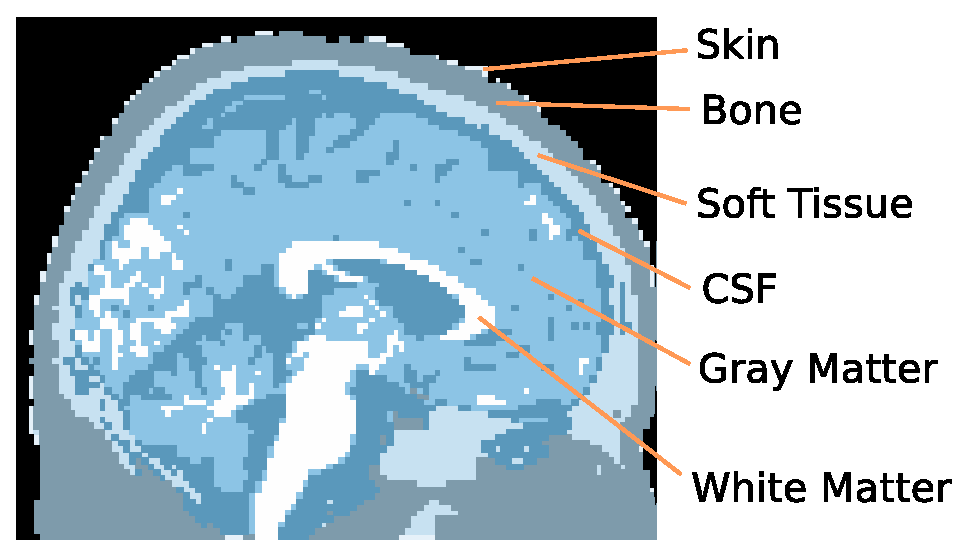
\includegraphics{segmented-head} 
    	\caption{\label{fig:segmented} Slice of the segmented head. Each color represents a different tissue type.} 
    \end{figure}
    \begin{table*}[tb] 
      \caption[Tissue-specific parameters]{\label{tbl:tissues} Tissue-specific parameters used to calculate the temperature change (from~\citet{collins}).} 
      \vspace{10pt}
      \small
    		\begin{tabular*}{\linewidth}{@{} l p{2.7cm}p{2cm}p{2.4cm}p{2.5cm}p{2cm}@{}}
    		  \toprule
    		  Tissue & $f_0$ \newline $100 \; ml/(g \; min)$ & $\rho$ \newline $kg/m^{3}$ & $c$ \newline $J \: kg^{-1} \: \degree C^{-1}$ & $k$ \newline $W \: m^{-1} \: \degree C^{-1}$ & $Q_{m}$ \newline $W/m^{3}$ \\
    		  \midrule
    			Bone & 3 & 1,080 & 2,110 & 0.65 & 26.1 \\
    			Cerebrospinal Fluid & 0 & 1,007 & 3,800 & 0.50 & 0 \\
    			Gray Matter & 67.1 & 1,035.5 & 3,680 & 0.565 & 15,575 \\
    			White Matter & 23.7 & 1,027.4 & 3,600 & 0.503 & 5,192 \\
    			Muscle & 3.8 & 1,041 & 3,720 & 0.4975 & 687 \\
    			Skin & 12 & 1,100 & 3,150 & 0.342 & 1,100 \\
    			\bottomrule
    		\end{tabular*}
    \end{table*}
  In order to begin the temperature calculating procedure, a model of the head must first be created.  Using SPM8 (\url{http://www.fil.ion.ucl.ac.uk/spm/}), we segmented a T1 contrast image of the head into five different tissue types: bone, cerebral spinal fluid, gray matter, white matter and soft tissue.  It was assumed that soft tissue voxels that are in contact with air are more appropriately labeled as skin, so in total we are left with a model of the head separated in to six tissue types (\cref{fig:segmented}).  The advantage this has is that we are able to use tissue specific parameters when doing the calculations, thereby improving the accuracy of the results.  The parameters used are available in~\cref{tbl:tissues}.  The code used to create the head matrix is discussed in~\cref{sec:headmatrix}.

  
  % CALC EQUIL T
    \subsection{\label{sec:calcequilT} Calculating the equilibrium temperature}
  The first step in calculating the temperature change is to first know what the resting state temperature is for each voxel within the head. Our approach was to have the initial temperature for all tissue voxels to be equal to 37\degree C and air voxels are kept at 24\degree C.  The starting temperature of the tissue doesn't affect the final resting state temperature; however, starting off at drastically different values could greatly increase the calculating time required before the temperature stabilizes. The finite difference implementation of the Pennes bioheat equation (\cref{eq:3dbioheat}) is used to update the temperature.  The temperature is updated until the temperature for every voxel has stabilized ($\frac{dT}{dt} < 10^{-6}$ \degree C/s).  Since temperature changes due to changes in neuronal activity are typically greater than $10^{-2}$ \degree C, a change in temperature less than $10^{-6}$ \degree C/s is sufficiently small that transient temperature changes are negligible and temperature can be considered stabilized.  The code used to calculate the equilibrium temperature is detailed in~\cref{sec:findequil}.
  
  % CALC M AND F
    \subsection{\label{sec:calcmf} Calculating Metabolism and Blood Flow Changes from fMRI BOLD}
    %%%%  Table of values used in Sotero, 2011  %%%%%
    \begin{table*}[bt]
      \caption[Parameters used in the single-voxel approximation]{\label{tbl:soteroparams} Parameters used to solve the single-voxel Penne's Bioheat Equation.  (modified from~\citet{sotero2011})}
      \small
        \begin{tabular*}{\linewidth}{lp{10cm}p{4cm}}
          \toprule
          Parameter & Meaning & Value \\
          \midrule
          T$_{a}$ & Arterial blood temperature & 37\degree C \\
          $C_{tissue}$ & Tissue Heat Capacity & 3.664 J/(gK) \\
          $\Delta H^{\circ}$ & Enthalpy released by oxidation of glucose & $4.7 10^{5}$ J \\
          $\Delta H_{b}$ & Enthalpy used to release O$_{2}$ from hemoglobin & $2.8 10^{4}$ J \\
          CMRO$_{2}\mid_{0}$ & Cerebral metabolic rate of O$_{2}$ consumption at rest & $0.0263 10^{-6}$ mol/(gs) \\
          CBF$\mid_{0}$ & Cerebral blood flow at rest & 0.0093 cm\textsuperscript{3}/(gs) \\
          $\rho_{b}$ & Blood density & 1.05 g/cm\textsuperscript{3} \\
          C$_{B}$ & Blood heat capacity & 3.894 J/(gK) \\
          $\tau$ & Time constant for conductive heat loss from the ROI to the surrounding tissue & 190.52 s \\
          a, b, c & Parameters of the gamma function fitted from E(f) vs. f & 0.4492, 0.2216, $-0.9872$ \\
          A & Maximum BOLD signal change & 0.22 \\
          $\alpha$ & Steady state flow-volume relation & 0.4 \\
          $\beta$ & Field-strength dependent parameter & 1.5 \\
          \midrule
          Variable & Meaning & \\
          \midrule
          m(t) & CMRO$_2$ normalized to baseline & \\
          f(t) & CBF normalized to baseline & \\
          T(t) & Temperature & \\
          W(t) & Lambert W Function & \\
          $\frac{\Delta S(t)}{S_0}$ & Change in BOLD signal normalized to rest & \\
          \bottomrule
        \end{tabular*}
    \end{table*}
    This is the critical step where we use fMRI BOLD data to calculate the normalized change in metabolism and blood flow.  The method used~\citep{sotero2011} is an assemblage of a couple other works [CITATION NEEDED]. It starts by using the relation between metabolism and blood flow proposed by~\citet{buxton2004}:
    \begin{equation} \label{eq:mf}
      m(t)=f(t)\frac{E(t)}{E_0}
    \end{equation}
  where $E_0$ is the oxygen extraction at rest and $E(f)$ is
    \begin{equation} \label{eq:E}
      E(f)=1-(1-E_0)^{\frac{1}{f(t)}}
    \end{equation}
  in accordance with the oxygen limitation model~\citep{buxton1997}.  Combining~\cref{eq:mf} with~\cref{eq:E} yields
    \begin{equation} \label{eq:EmfCombined}
      m(t)=\frac{f(t)}{E_0}\left[1-(1-E_0)^{\frac{1}{f(t)}}\right]
    \end{equation}
  \Citet{sotero2011} goes about solving~\cref{eq:EmfCombined} by adjusting $E(t)$ data generated by~\cref{eq:E} and fitting it to the gamma function for the $f$ range (0.7--2.0) that is within experimentally reported values~\citep{fox1988,leithner2009,lin2010}:
    \begin{equation} \label{eq:gammafct}
      \frac{E(f)}{E_0}=af^{c}(t)e^{-bf(t)}
    \end{equation}
  where values for a, b and c are provided in~\cref{tbl:soteroparams}.  From this approximation we have the final form of metabolism:
    \begin{equation} \label{eq:m} 
      m(t)=af^{c+1}(t)e^{-bf(t)}.
    \end{equation}
  As proposed by~\citet{davis1998}, the BOLD signal changes ($\frac{\Delta S(t)}{S_0}$) can be described in terms of $m(t)$ and $f(t)$:
    \begin{equation} \label{eq:S}
      \frac{\Delta S(t)}{S_0} = \frac{S(t)-S_0}{S_0} = A(1-f^{\alpha-\beta}(t) m^\beta(t))
    \end{equation}
  Substituting~\cref{eq:m} into~\cref{eq:S} yields
    \begin{equation} \label{eq:mAndS}
      f(t)e^{-\frac{b \beta}{\alpha + \beta c}f(t)}=\left(\frac{\left(A-\frac{\Delta S(t)}{S_0}\right)}{A a^\beta}\right)^{\frac{1}{\alpha+\beta c}}
    \end{equation}
  where A is the maximum change in BOLD signal.  Multiplying each side by $-\frac{b\beta}{\alpha+\beta c}$ gives
    \begin{equation} \label{eq:mAndSmultiplied}
      -\frac{b\beta}{\alpha+\beta c} f(t)e^{-\frac{b \beta}{\alpha + \beta c}f(t)}=-\frac{b\beta}{\alpha+\beta c} \left(\frac{\left(A-\frac{\Delta S(t)}{S_0}\right)}{A a^\beta}\right)^{\frac{1}{\alpha+\beta c}}
    \end{equation}
  which can be solved by using the Lambert W function
    \begin{equation} \label{eq:lambertW}
      z=W(x)
    \end{equation}
  where z is given by
    \begin{equation} \label{eq:lambertWsetup}
      z e^z = x
    \end{equation}
  Finally, $f(t)$ is obtained from~\cref{eq:mAndSmultiplied}
    \begin{equation} \label{eq:f}
      f(t)=\frac{\alpha+\beta c}{b \beta}W(y(t))
    \end{equation}
  where
    \begin{equation} \label{eq:y} 
    	y(t)=-\frac{b \beta}{\alpha+\beta c} \left[\frac{(A-\frac{S(t)}{S_{0}}-1)}{A a^{\beta}}\right]^{\left(\frac{1}{\alpha+\beta c}\right)} 
    \end{equation}
  is a function of the BOLD signal.  Using \cref{eq:m,eq:f,eq:y} allows for the metabolism and blood flow to be calculated from the BOLD signal (values used are provided in~\cref{tbl:soteroparams}).
  
    In order to process the files, the input BOLD data is stored in folder as a separate file for each time step.  The first step in processing the data for temperature calculations is to determine a resting state BOLD signal ($S_0$).  The resting state is calculated by taking the element-wise mean of the data when the subject is at rest (i.e. the first and last 20 seconds).  This results in one data set where each voxel is a mean of all of the voxels at the location over time ($S_0$).  In order to calculate the metabolism and blood flow, the BOLD dataset needs to be normalized to this resting state ($\frac{\Delta S(t)}{S_0}$).  
    
    Once $\frac{\Delta S(t)}{S_0}$ is known for each time step, \cref{eq:m,eq:f,eq:y} can be used to calculate the metabolism and blood flow. The implementation of these functions is available in~\cref{sec:fmriprocessing}. 

  % CALC CHANGE IN T
    \subsection{\label{sec:calcT} Calculating the change in temperature in the active brain}
% RESULTS
  \section{\label{sec:results} Results} 
  %% THEORETICAL RESULTS %%
    \subsection{\label{sec:theoreticalresults} Using Theoretical BOLD Data}
    \FloatBarrier
    \begin{figure}[p] 
    	\begin{center}
    		\begin{tabularx}{\textwidth}{cc}
    			\raisebox{20px}{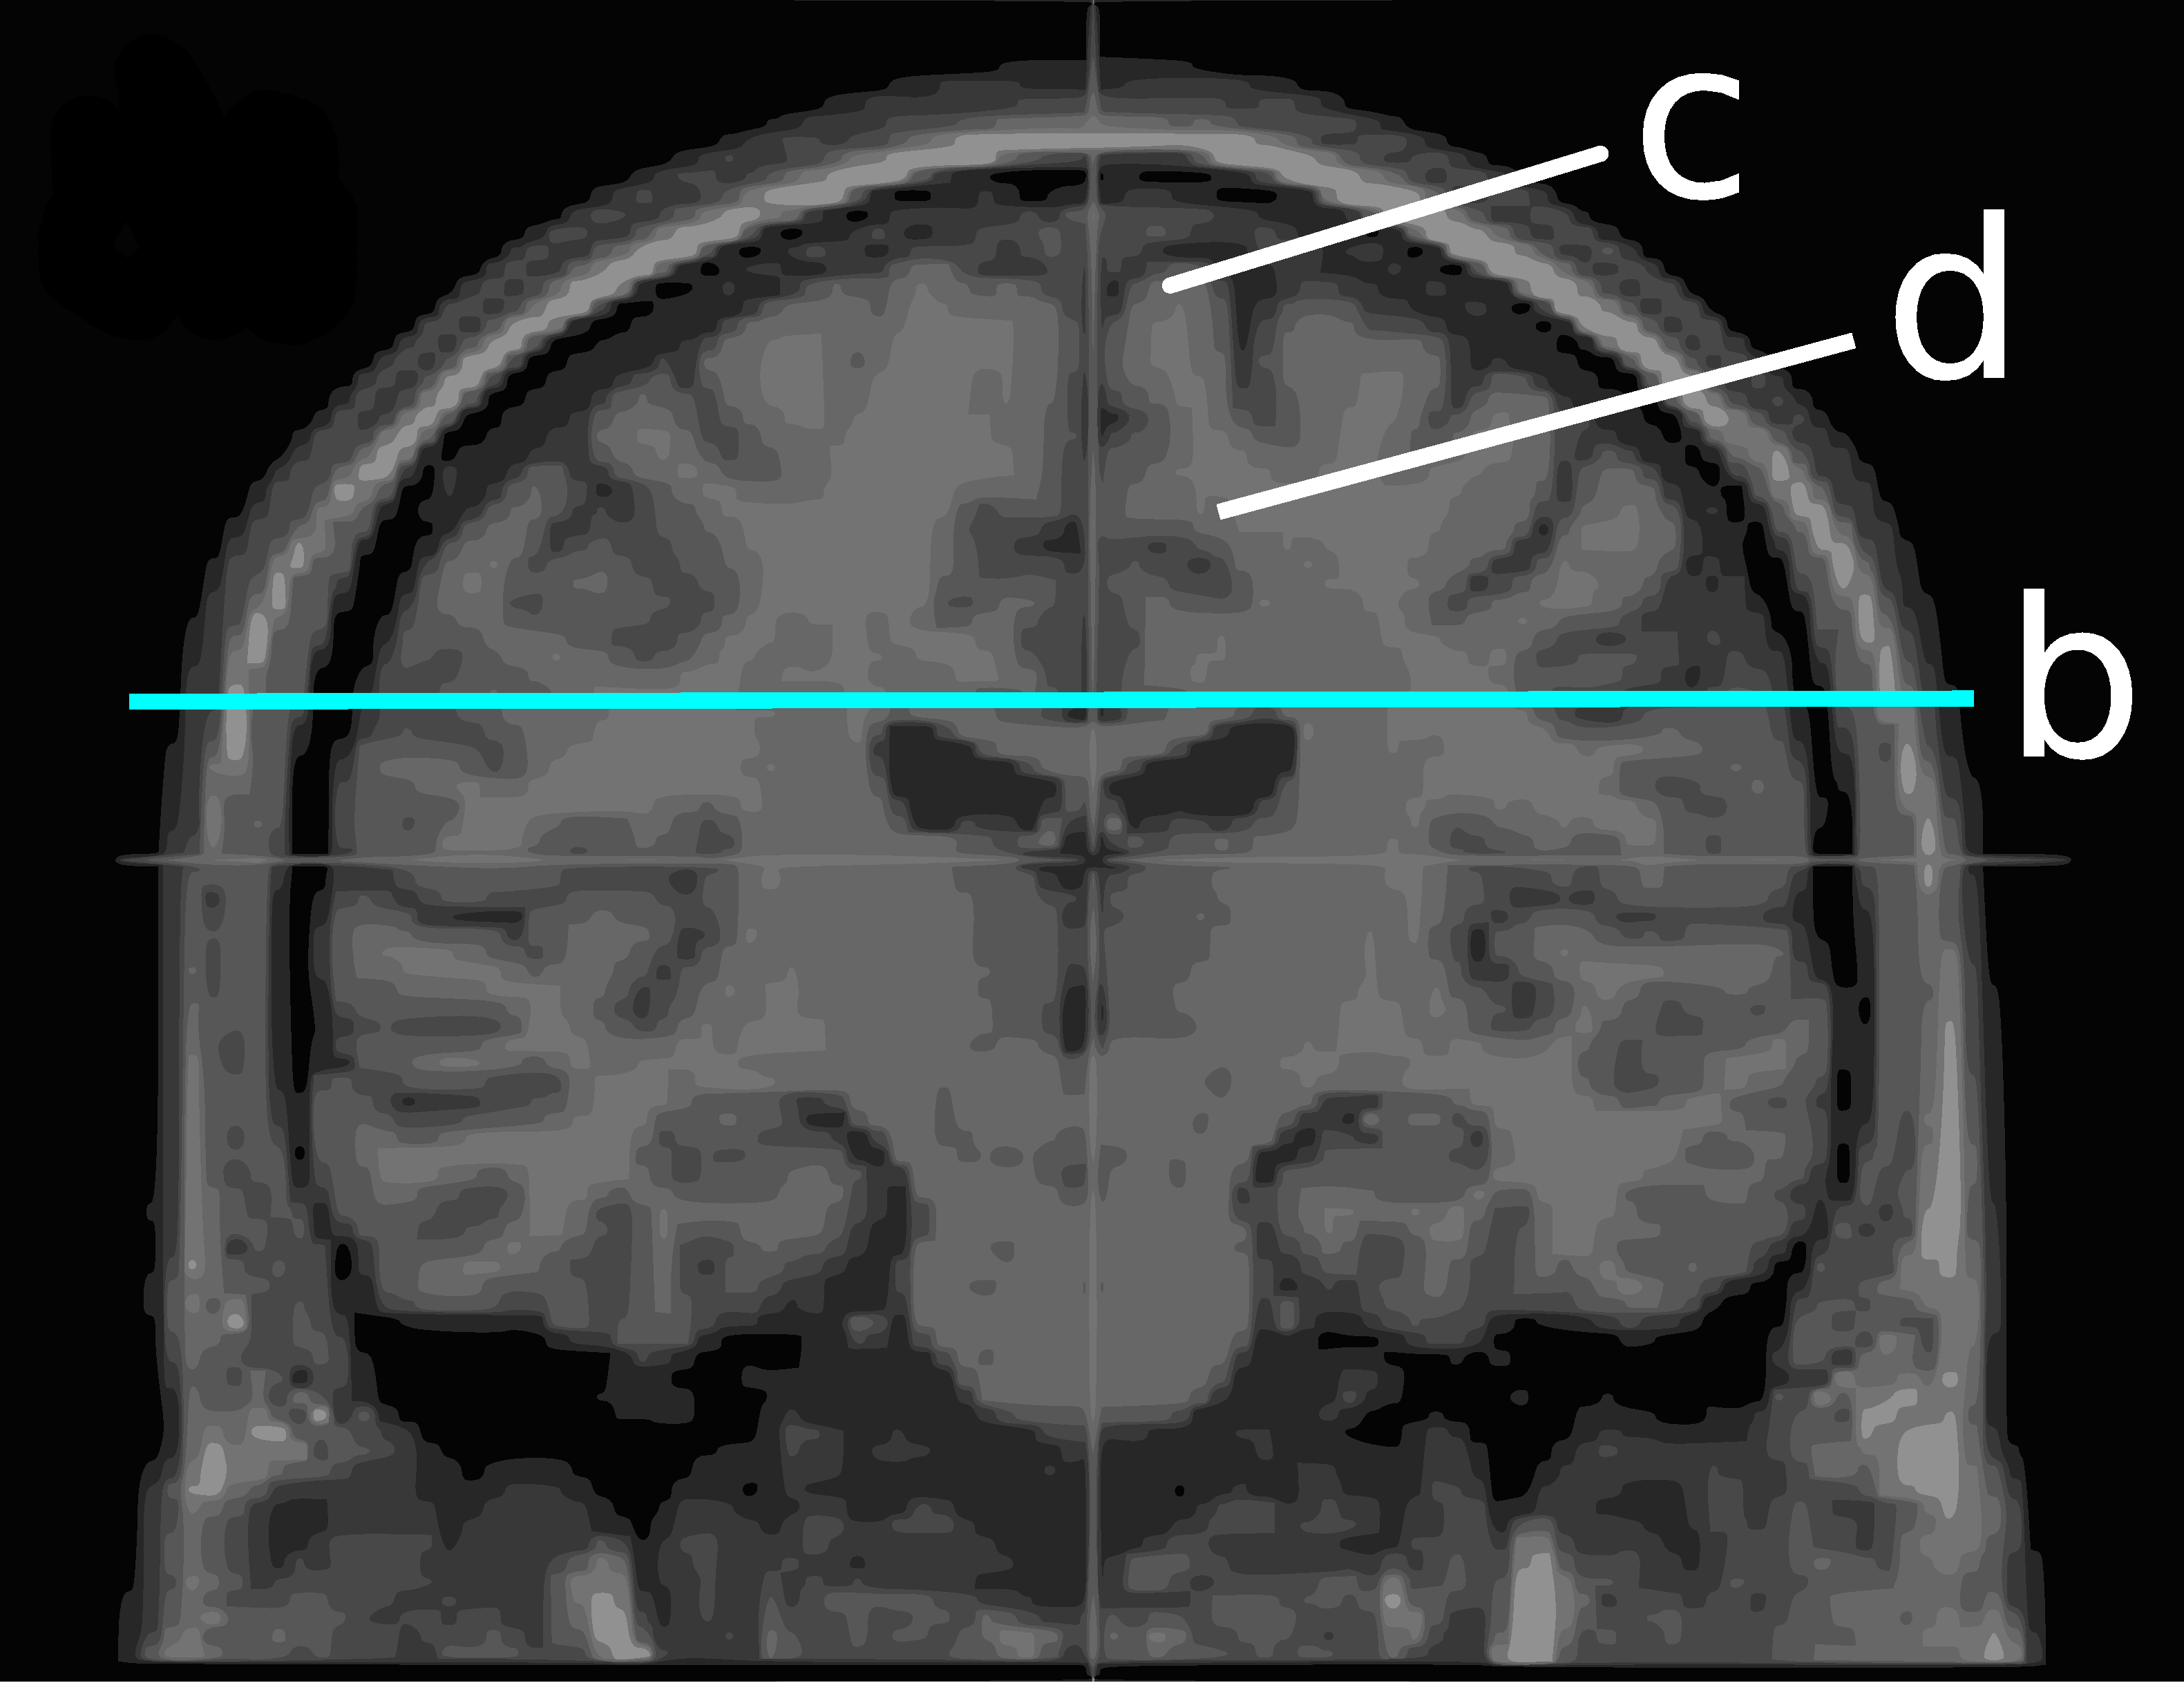
\includegraphics[width=0.36\textwidth]{headref}} & 
    			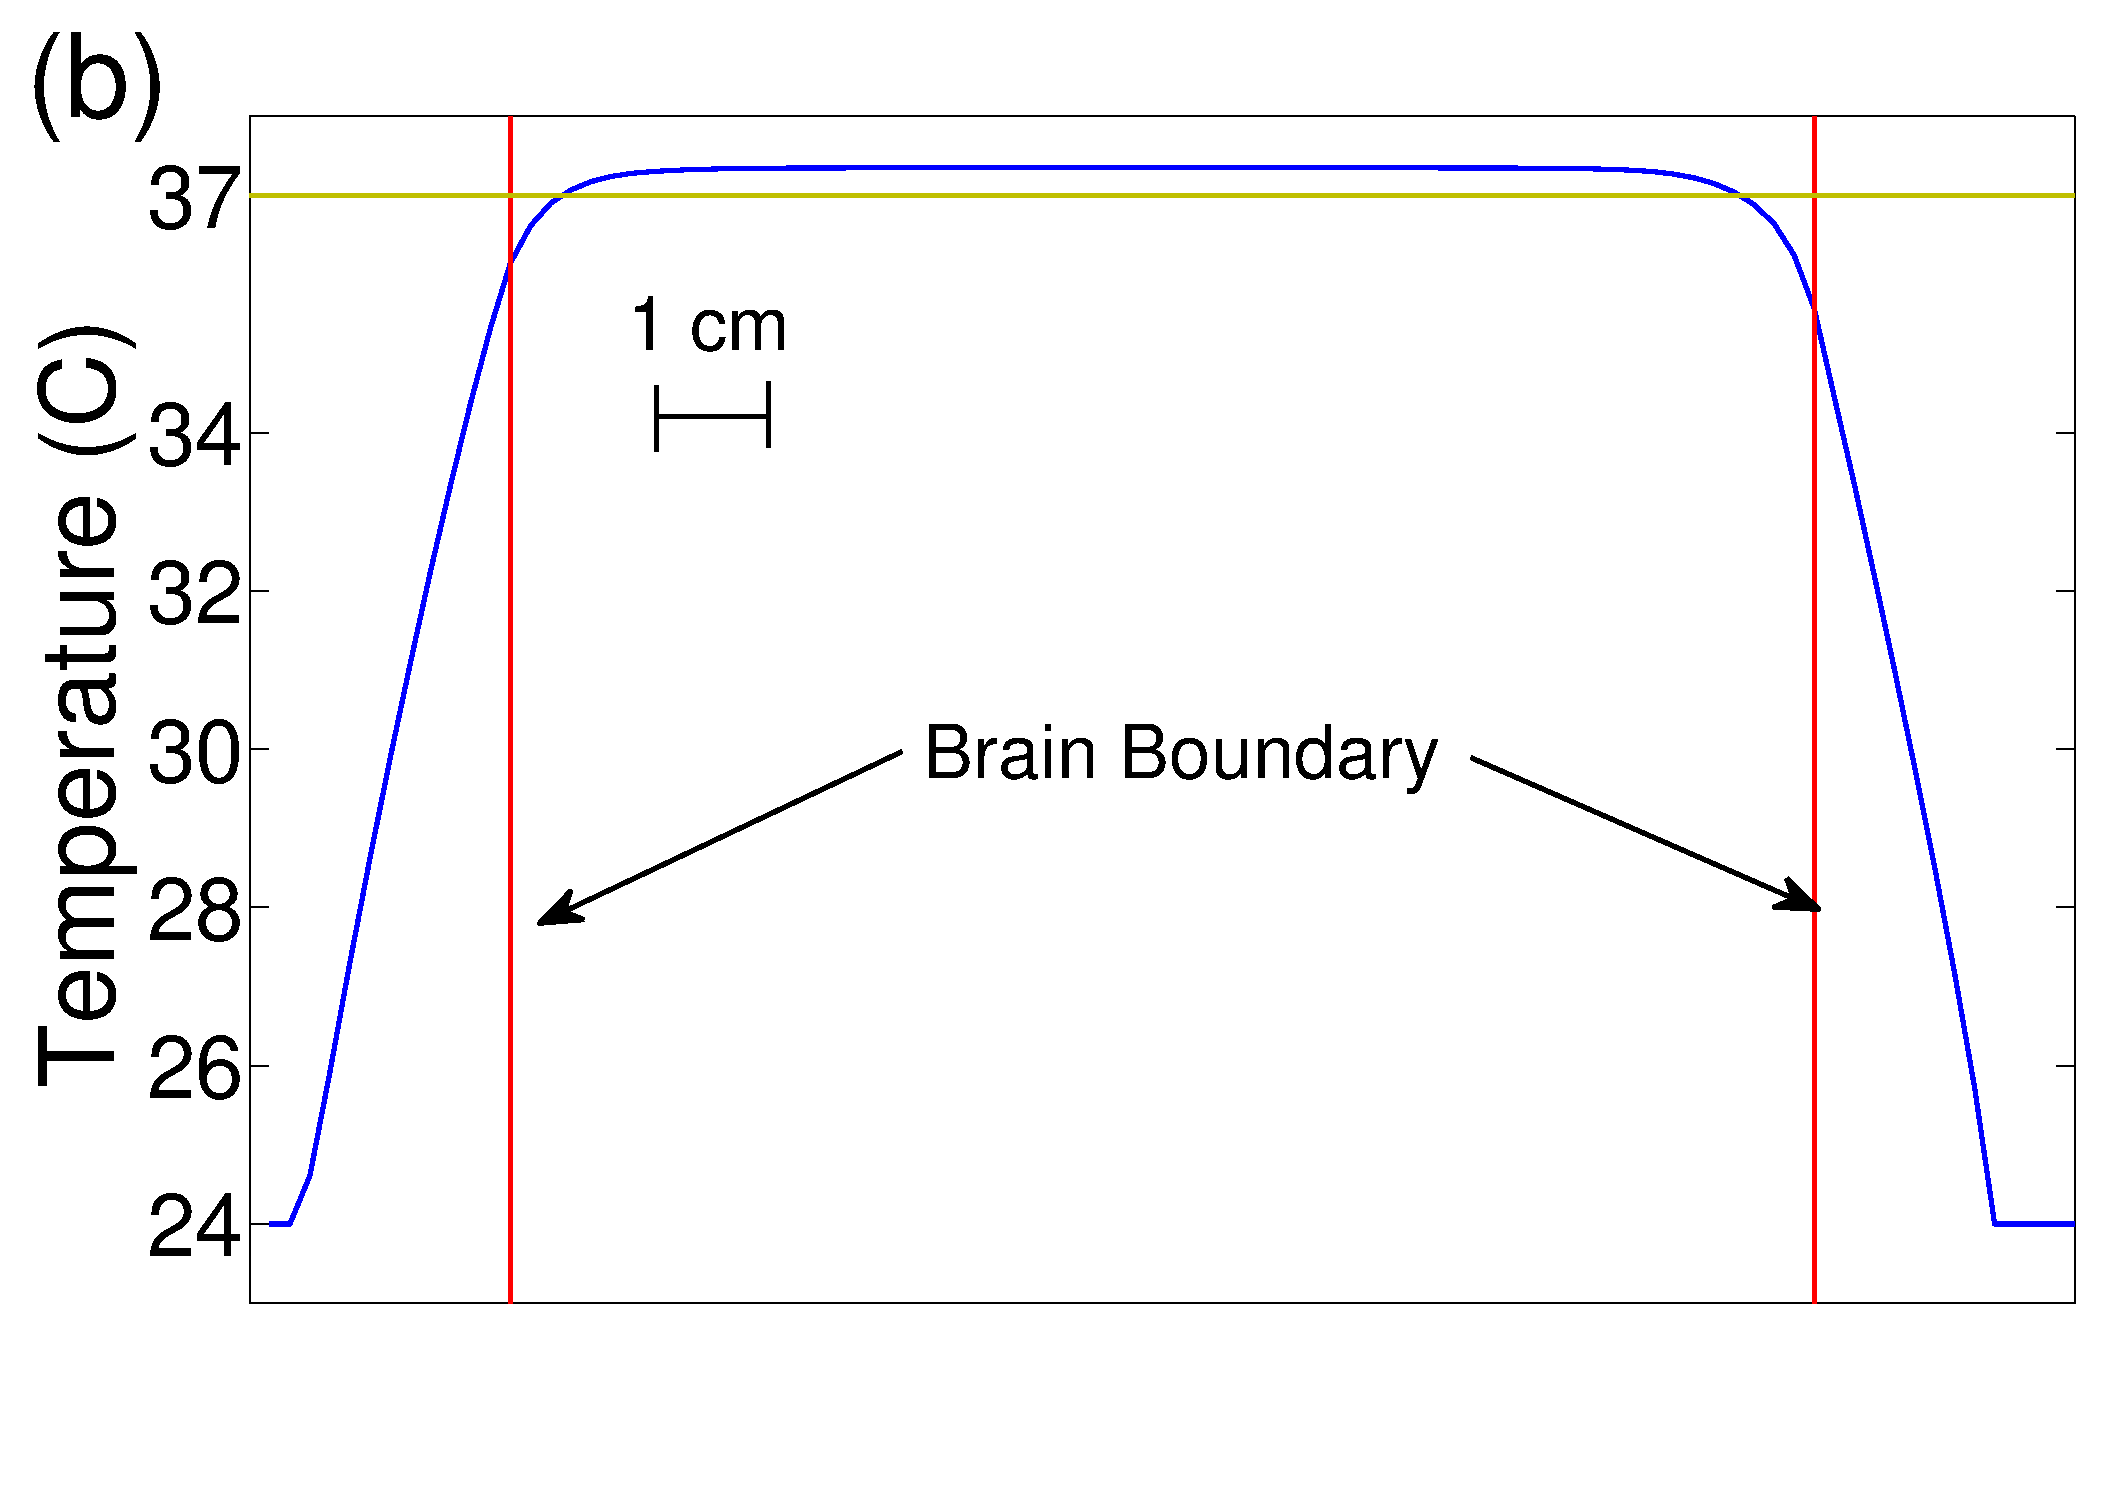
\includegraphics[width=0.5\textwidth]{equilibrium_temperature_0_55_52} \\
    			\multicolumn{2}{c}{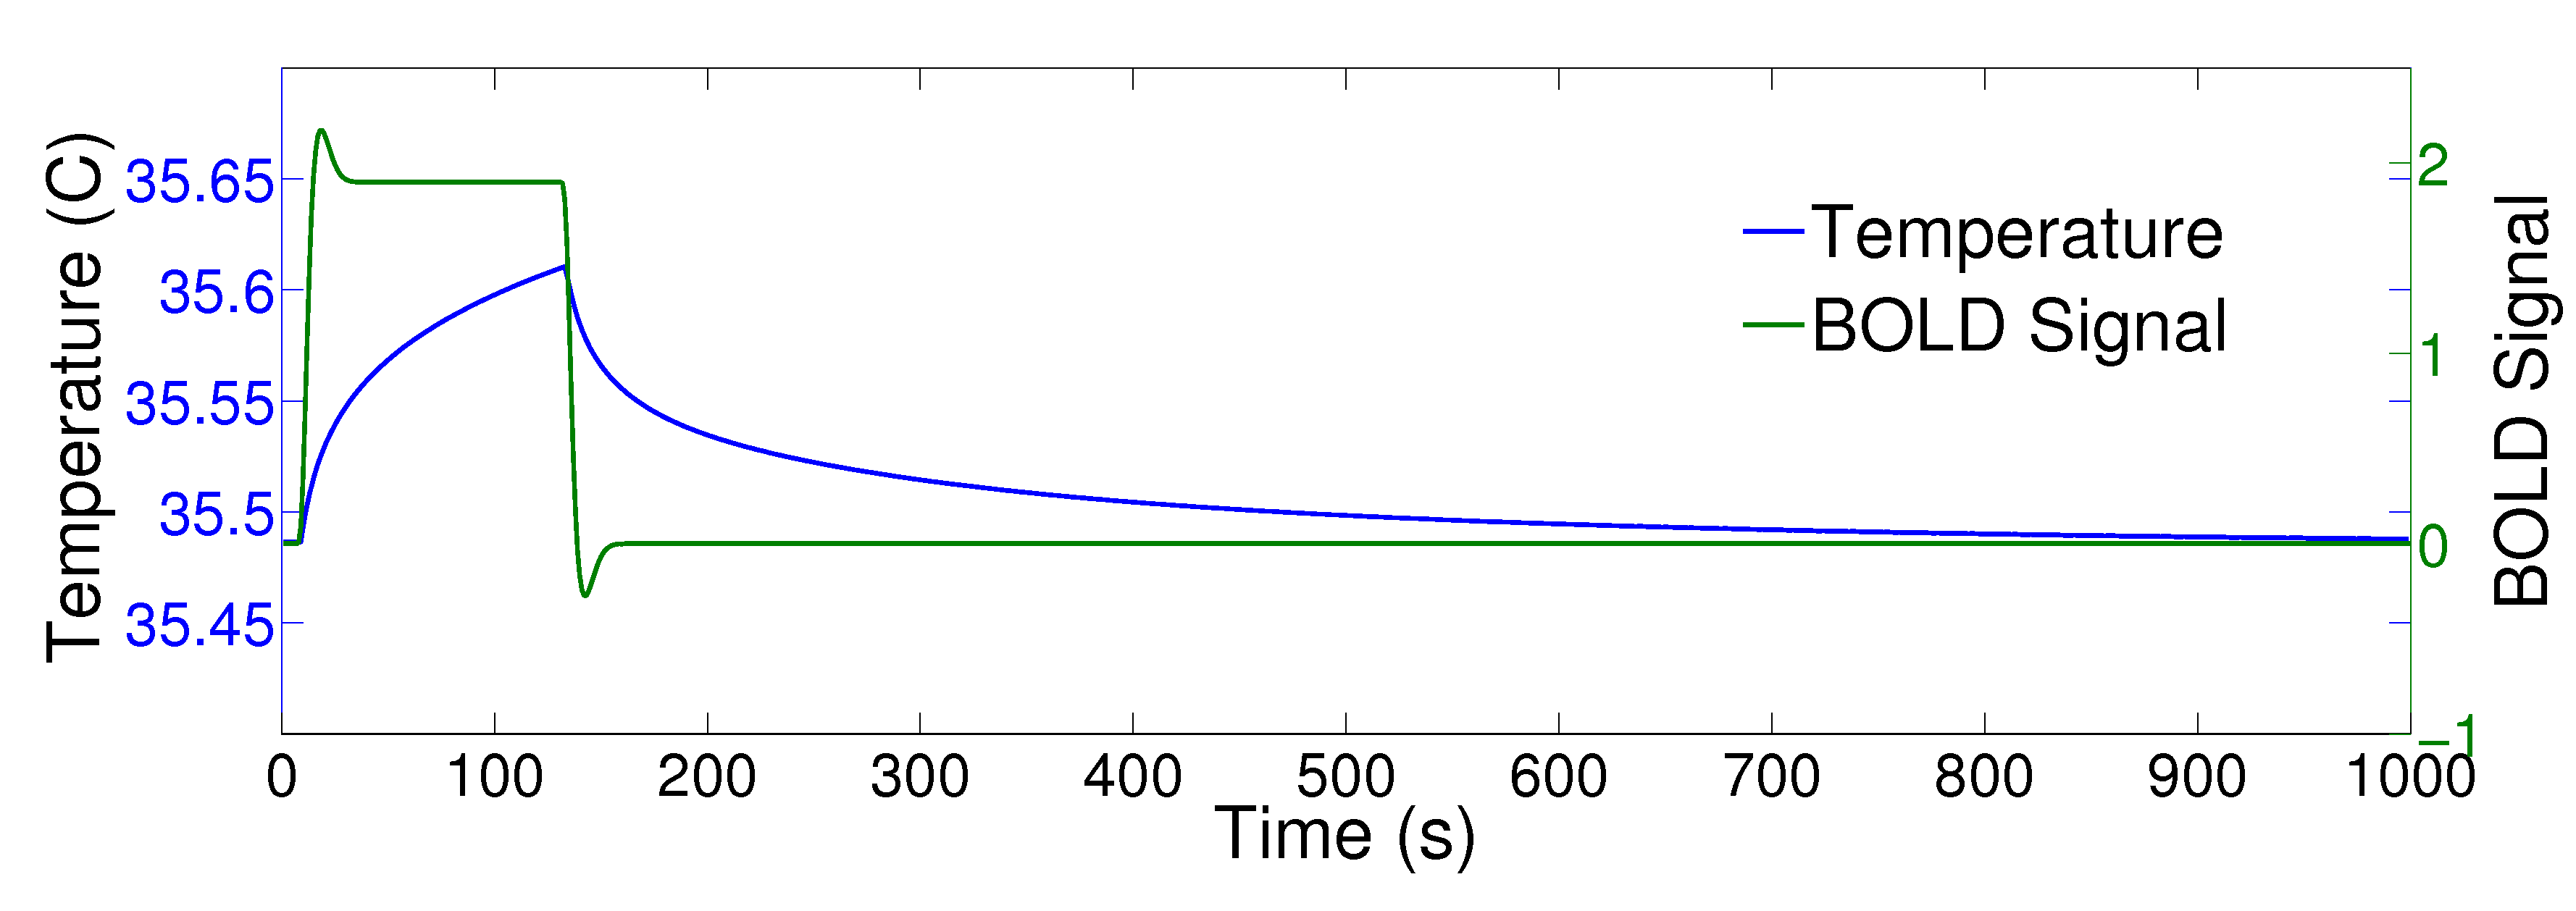
\includegraphics{sim_bold_(48_58_76)}} \\
    			\multicolumn{2}{c}{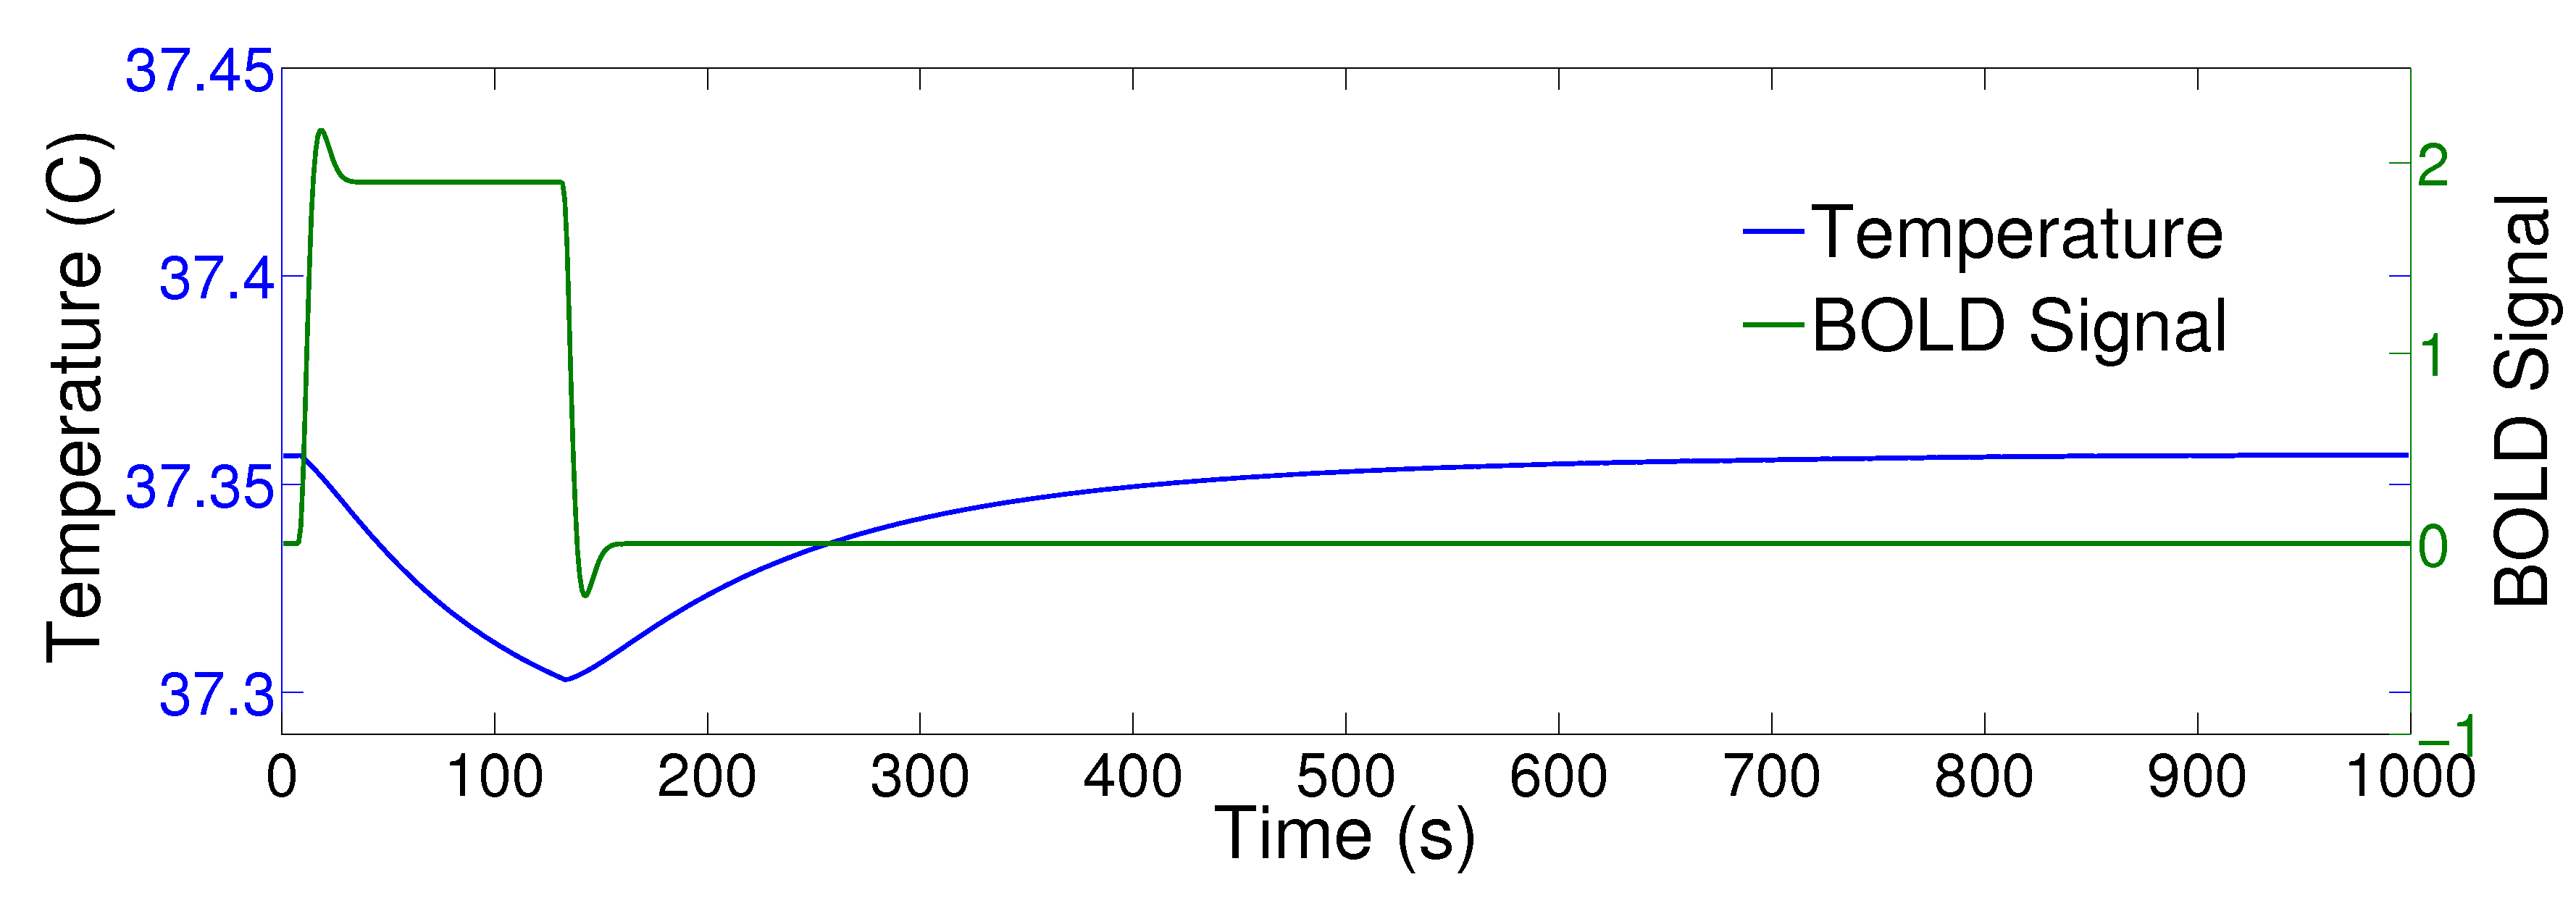
\includegraphics{sim_bold_(48_58_56)}}
    		\end{tabularx}
    	\end{center}
    	\caption[Temperature changes: simulated BOLD data]{\label{fig:simulateddata} Temperature changes using simulated BOLD signals. (a) Slice of the head (y = -12) with indicators of the locations for parts (b)-(d). (b) Equilibrium temperature along a line through the head. Red lines indicate the brain boundary and the gold line indicates the blood temperature (37\degree C) used for calculations. Inside the brain, a 4-6 mm thick shell is created where the equilibrium temperature is less than the blood temperature. Within this shell, (c) the temperature rises with increased brain activity while (d) tissue deeper in the brain experiences the opposite effect.} 
    \end{figure}
    %%  EXPERIMENTAl RESULTS %%
    \subsection{\label{sec:experimentalresults} Using Experimental BOLD Data}
    \FloatBarrier
    \begin{figure}[p] 
    	\begin{center}
    		$ 
    		\begin{array}{c}
    			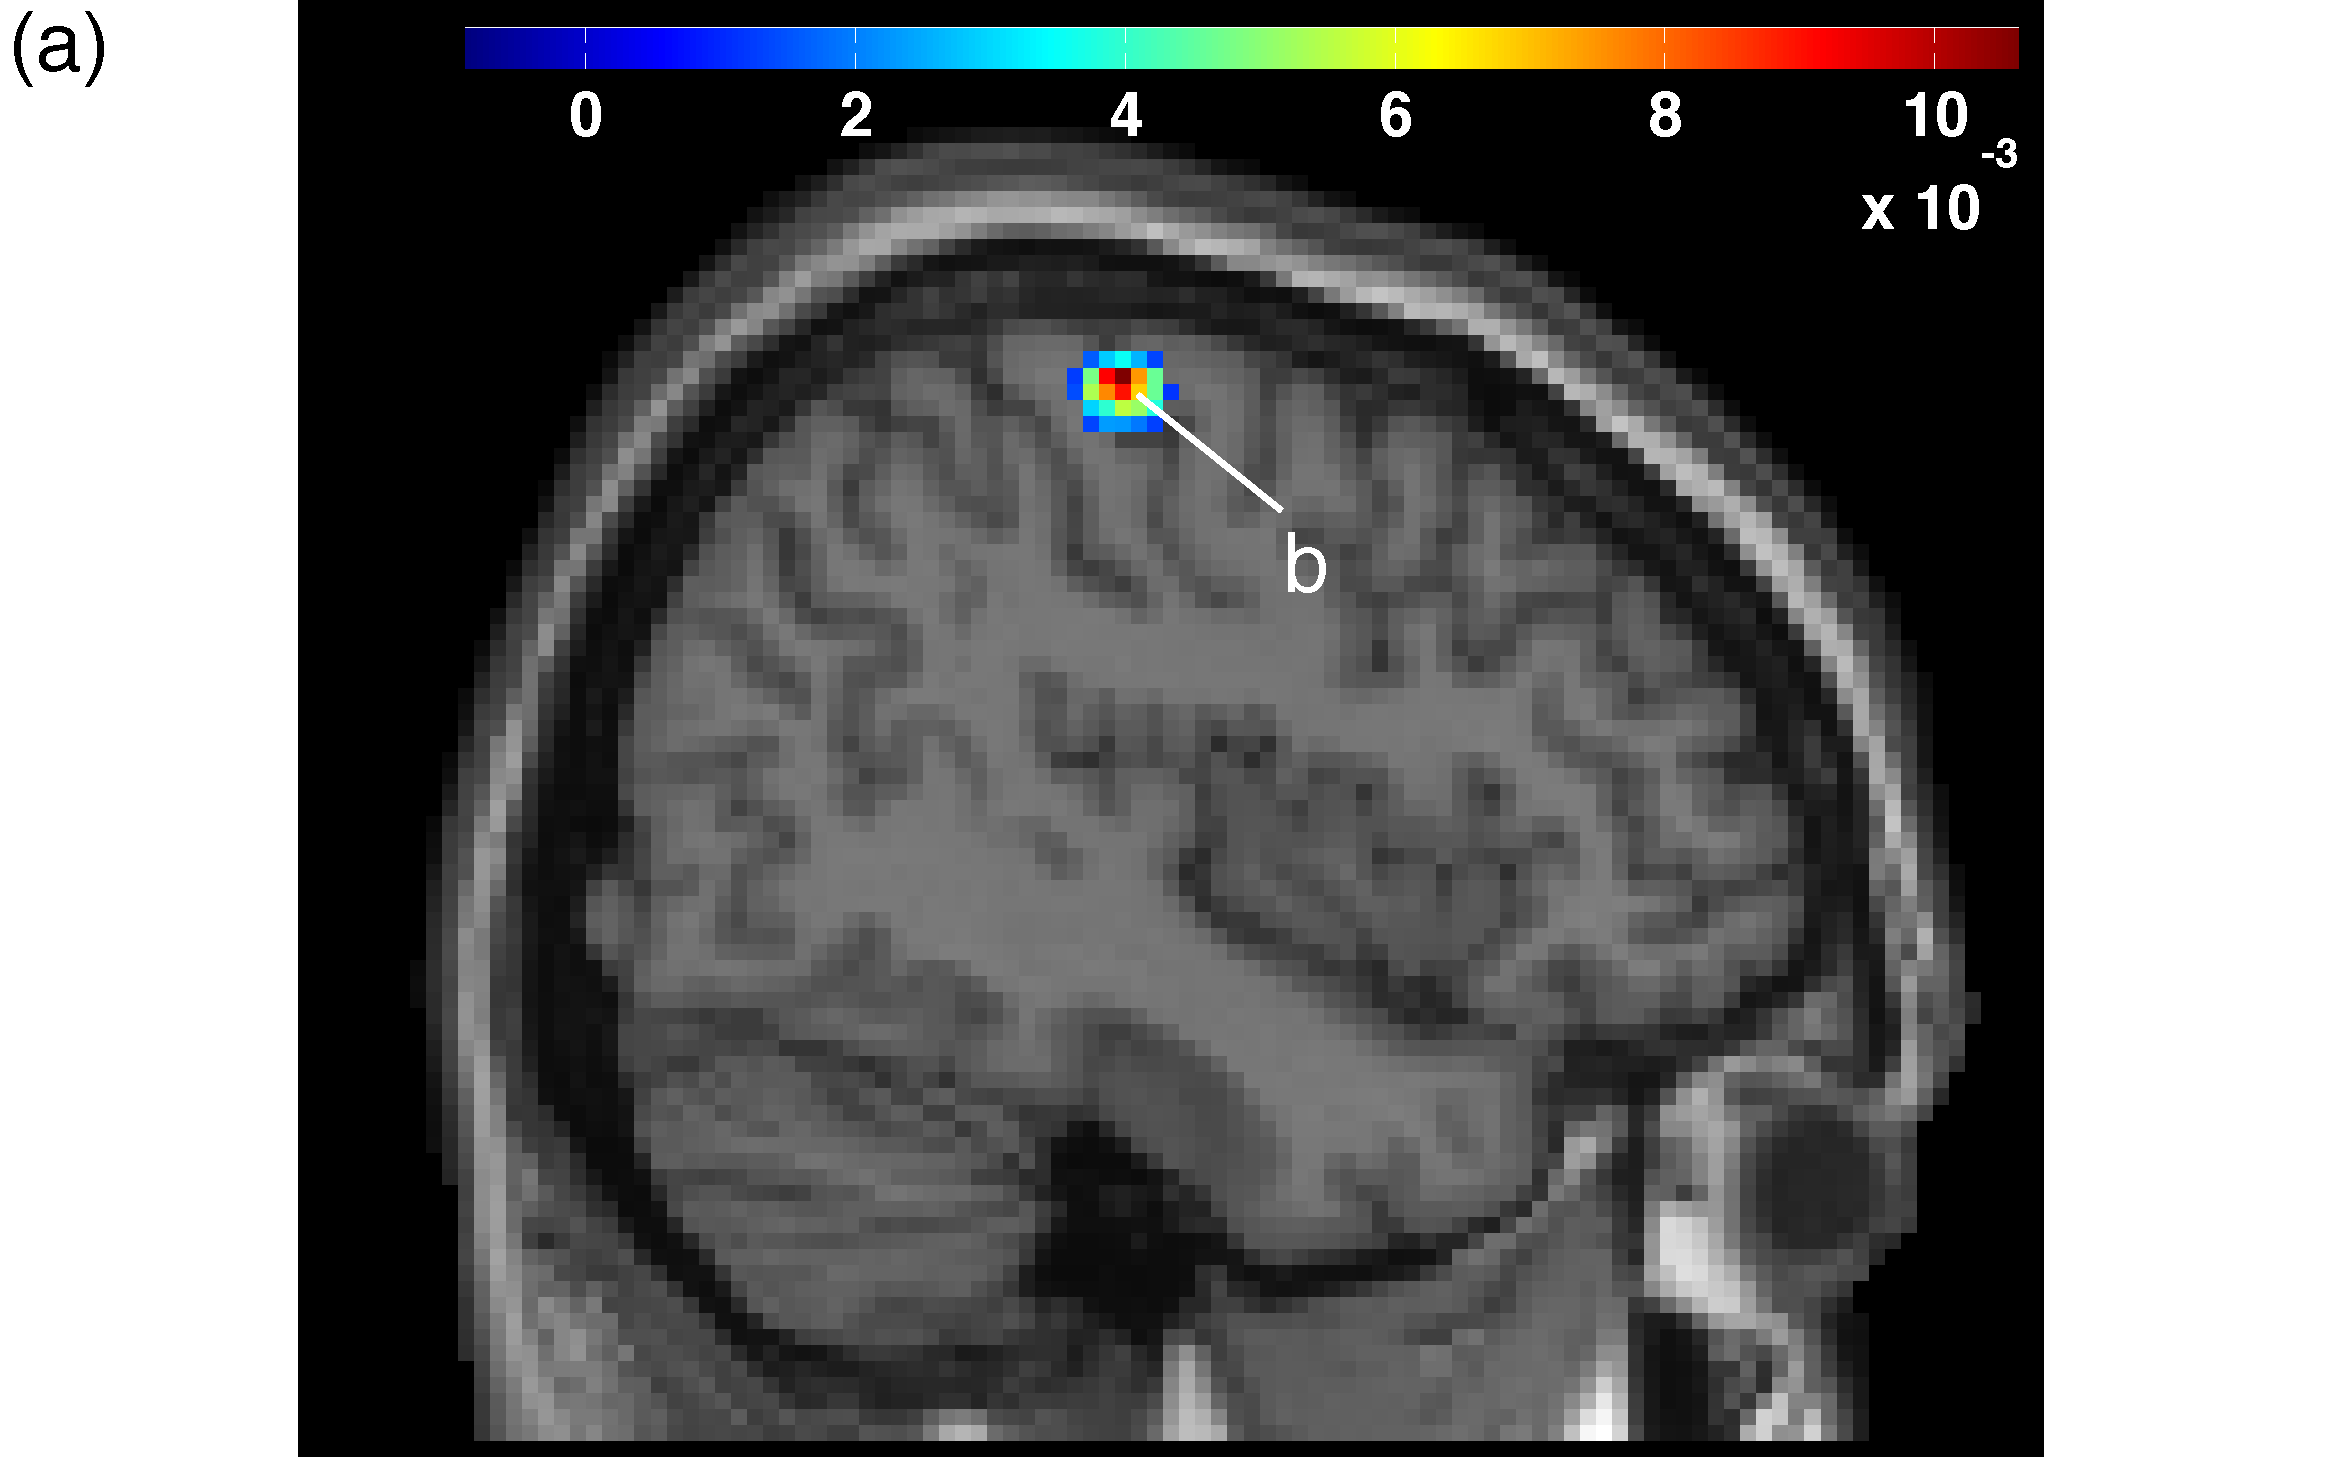
\includegraphics[width=0.9\linewidth]{slice_x_24} \\
    			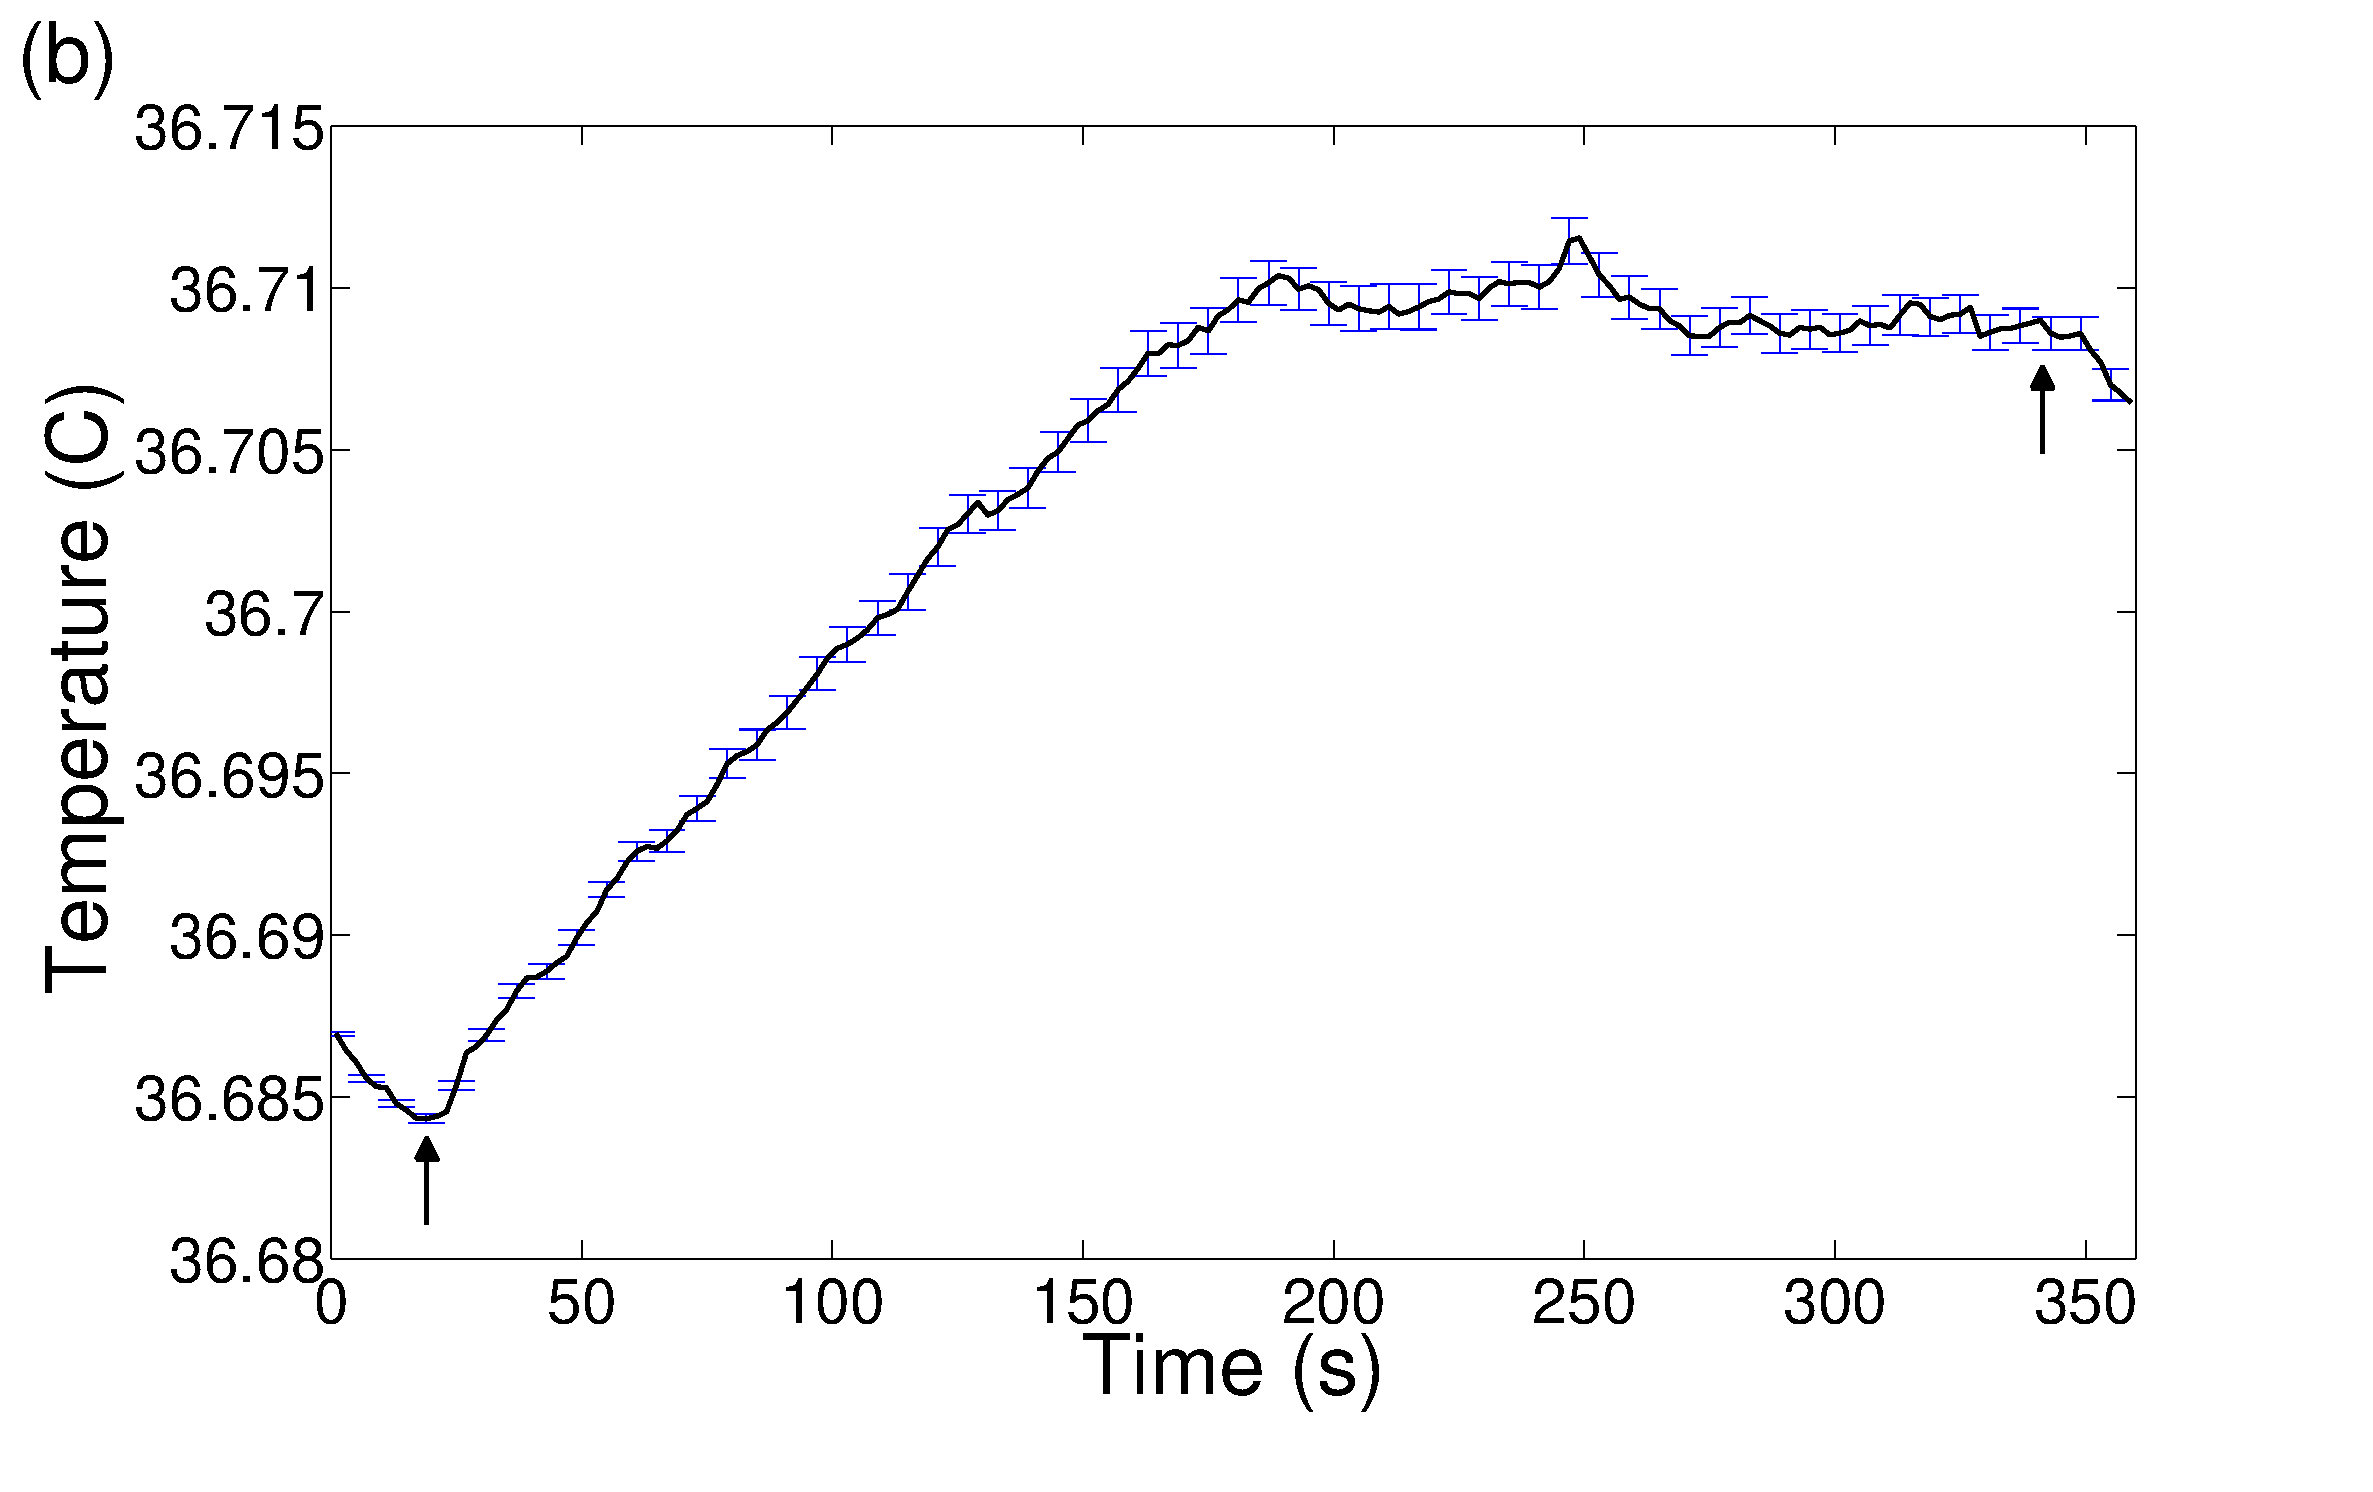
\includegraphics[width=0.9\linewidth]{avg_data_24_52_67} 
    		\end{array}
    		$ 
    	\end{center}
    	\caption[Temperature changes: experimental BOLD data]{\label{fig:realdata} Temperature calculated from a voxel within the motor cortex. (a) A slice (x = -44) showing the motor cortex warming during a finger-tapping task. (b) Temperature at a voxel within the motor cortex (-44, -24, 60) with standard error indicated by blue error bars (Arrows indicate task onset and conclusion, N=24).} 
    \end{figure}
  % talk about my approach